% Résultats : références, modèles, ablations, test scellé, marché.
% Chiffres recopiés des pages générées docs/resultats/ (references.md, modeles.md, ablations.md,
% test_scelle_h1.md) ; log-loss en nats par match.

\chapter{Résultats}
\label{chap:resultats}

\section{Références}

Sur les 7\,156 matchs des quatre plis, B0 (même loi pour tous) a un log-loss de 1,9029 et B1 (moyennes
du championnat par terrain) de 1,8984 : connaître le championnat et le terrain fait gagner 0,0046 nat par
match (\([0{,}0010 ; 0{,}0080]\)), soit 0,24~\%. C'est l'ordre de grandeur attendu pour une variable aussi
bruitée. Le marché avant clôture est loin devant sur l'événement plus ou moins 2,5 buts : Brier de 0,2387
contre 0,2478 pour B1 ; la clôture fait encore mieux (0,2374), signe que de l'information arrive jusqu'au
coup d'envoi.

\section{Structures de modèles}
\label{sec:resultats-modeles}

Avec les mêmes variables (G0 et G1), sur les 4 plis :

\begin{center}
\begin{tabular}{lcccl}
\toprule
Modèle & Log-loss & RPS & Brier \(P(T > 2{,}5)\) & Lecture \\
\midrule
B0 & 1,9029 & 0,1320 & 0,2491 & référence \\
B1 & 1,8984 & 0,1313 & 0,2478 & référence à battre \\
M1, linéaire & 1,9092 & 0,1309 & 0,2471 & moins bon que B1 \\
M2, Poisson sur le total & 1,8930 & 0,1305 & 0,2460 & bat B1 \\
M3, Poisson par équipe & 1,8897 & 0,1301 & 0,2450 & \textbf{structure retenue} \\
M5, Dixon-Coles & 1,8897 & 0,1301 & 0,2450 & sans gain \\
\bottomrule
\end{tabular}
\end{center}

\begin{itemize}
  \item \textbf{La forme de la loi compte.} M1 a la bonne moyenne mais une loi normale : il met 2,5~\%
        de sa masse sur des totaux négatifs et sa variance est supposée constante, alors qu'elle croît
        avec la moyenne. Il perd contre B1 (\(-0{,}0108\), \([-0{,}0166 ; -0{,}0049]\)). M2, avec une loi
        de comptage, le bat de 0,0162.
  \item \textbf{Décomposer par équipe paie} : M3 bat M2 de 0,0033 (\([0{,}0014 ; 0{,}0052]\)), dans les
        4 plis, avec les mêmes variables.
  \item \textbf{Ni la dispersion ni la dépendance ne changent la loi du total.} Les buts d'une équipe
        sont même légèrement sous-dispersés une fois les variables connues (\(\hat\varphi \approx
        0{,}98\)) : la binomiale négative (M4) se confond avec Poisson et n'est pas évaluée. Dixon-Coles
        (M5) estime \(\rho \approx -0{,}06\) : il corrige \(P(T = 1)\) mais dépasse sur \(P(T = 0)\), pour
        un log-loss inchangé.
  \item \textbf{La régularisation n'apporte rien} : avec environ 33\,000 lignes pour une trentaine de
        coefficients, le ridge et l'élastique net font jeu égal avec le Poisson non régularisé (M6).
\end{itemize}

\section{Que rapporte chaque information ?}

Sur la structure M3, les groupes de variables s'ajoutent un à un (figure~\ref{fig:apport}) :

\begin{center}
\begin{tabular}{lccc}
\toprule
Étape & Log-loss & Apport de l'étape [IC 95~\%] & Retenu \\
\midrule
G0, contexte & 1,8990 & \(+0{,}0039\) sur B0 & oui \\
+ G1, Elo & 1,8897 & \(+0{,}0094\) \([0{,}0060 ; 0{,}0128]\) & oui \\
+ G2, glissants & 1,8805 & \(+0{,}0092\) \([0{,}0057 ; 0{,}0127]\) & oui \\
+ G3, calendrier & 1,8806 & \(-0{,}0001\) \([-0{,}0004 ; 0{,}0002]\) & non \\
\bottomrule
\end{tabular}
\end{center}

\begin{figure}[ht]
  \centering
  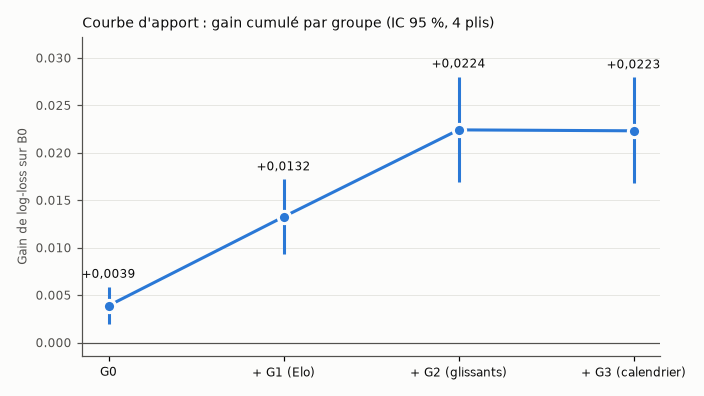
\includegraphics[width=0.75\textwidth]{figures/courbe_apport.png}
  \caption{Gain cumulé de log-loss sur B0 par groupe de variables, avec intervalle à 95~\% (4 plis,
           7\,156 matchs).}
  \label{fig:apport}
\end{figure}

L'Elo dit qui est fort ; les moyennes glissantes disent combien une équipe marque et encaisse, ce qui
est précisément la question du total : elles apportent presque autant que l'Elo. Le calendrier n'apporte
rien. Apprendre aussi sur les deuxièmes divisions ne fait pas mieux que le top 5 seul. Le
\textbf{modèle retenu} (ADR-0039) est donc M3 sur G0, G1 et G2, appris sur le top 5 : il bat B1 de
\(0{,}0179\) (\([0{,}0133 ; 0{,}0226]\)), dans les 4 plis, avec une pente de calibration de 0,95 et une
couverture de son intervalle à \(\pm 1{,}1\) point de l'annoncée.

\section{Test scellé}

Le test a été lancé une fois, sur 2\,092 matchs joués entre le 1\textsuperscript{er} juillet 2025 et le
18 octobre 2026. Un premier lancement a échoué pour une raison technique (une date mal encodée dans le
rapport), sans qu'aucun résultat soit affiché ; la relance unique a été décidée par écrit, avec ses
règles de lecture, puis contrôlée par l'empreinte des prédictions, identique au premier lancement
(ADR-0043).

\begin{center}
\begin{tabular}{lcccc}
\toprule
Modèle & Log-loss & RPS & Brier \(P(T > 2{,}5)\) & Couverture (annoncée) \\
\midrule
Modèle retenu & 1,8805 & 0,1281 & 0,2414 & 87,3~\% (87,5~\%) \\
B1 & 1,8994 & 0,1305 & 0,2457 & 88,3~\% (88,0~\%) \\
B0 & 1,9063 & 0,1316 & 0,2484 & 87,1~\% (87,4~\%) \\
\bottomrule
\end{tabular}
\end{center}

\begin{itemize}
  \item \textbf{Le modèle bat B1} : \(+0{,}0189\) (\([0{,}0102 ; 0{,}0282]\)), un gain du même ordre qu'en
        validation glissante. Il bat aussi B1 en RPS et en Brier.
  \item \textbf{Calibration} : pente de 1,00 ; couverture à 0,2 point de l'annoncée. Par décile de
        \(P(T > 2{,}5)\), l'écart moyen est de 2,5 points, mais la moitié des déciles dépassent 3 points
        (le plus grand : 5,7). Avec 209 matchs par décile, l'erreur d'échantillonnage seule est
        d'environ 3,5 points : ce critère est un diagnostic, publié tel quel (ADR-0037).
  \item \textbf{Le marché reste meilleur} sur l'événement plus ou moins 2,5 buts, sur les 2\,001 matchs
        qui ont une cote : Brier de 0,2418 pour le modèle, 0,2397 pour le marché avant clôture, 0,2383 à
        la clôture. Le modèle comble environ les deux tiers de l'écart entre B1 (0,2458) et le marché.
\end{itemize}

Après le test, aucun modèle H1 n'a été modifié. Le modèle final a été réappris par la même procédure sur
toutes les données, matchs scellés compris : 40\,180 lignes jusqu'au 18 octobre 2026, demi-vie de 240
jours, coefficients à 0,009 au plus de ceux du modèle testé (ADR-0044).
